The inflatable structure consists of three main design elements: The aerodynamic shape, structural arrangement and \gls{tps} design. These elements will be covered in the subsequent sections in the aforementioned order.

\paragraph{Aerodynamic shape}
The aeroshell will have a shape similar to configuration D in Figure \ref{fig:aeroshapes} in Section \ref{subsec:aerosens}, with a radius of $6$ $\left[m\right]$ and a half cone angle of approximately $\gls{sym:theta_cone} = 70 \left[deg\right]$. The curved nose will have an outer radius of $2.5 \left[m\right]$. The cross-sectional offset at the rear of the body is approximately $0.91 \left[m\right]$. At an angle of attack of $\gls{sym:alpha} = 22.5 left[deg\right]$, it has a lift-to-drag ratio of $\gls{sym:L} \cdot \gls{sym:D}^{-1} = 0.35\left[-\right]$ and a drag coefficient of $\gls{sym:CD} = 1.3 \left[-\right]$. At this angle of attack, a \gls{cg}-offset of $\gls{sym:CM}\cdot \gls{sym:lref} \cdot \gls{sym:CX}^{-1} = 0.5 \left[m\right]$ is required to trim the vehicle around the pitch axis. It has a moment derivative of $\gls{sym:cm-alpha} = -0.21 \left[rad^{-1}\right]$. 

 Figures \ref{fig:aeroshape.frontview} through \ref{fig:aeroshape.isoview} show the final \gls{oml} of the aeroshell. The final shape is composed of circular cross-sections stacked on top of each other, with an offset in the $z$-direction. The aeroshell is $1.8 \left[m\right]$ high and has a maximum offset of $0.9 \left[m\right]$.
 
\begin{figure}[h]
	\centering
	
	\begin{subfigure}[b]{0.49\textwidth}
		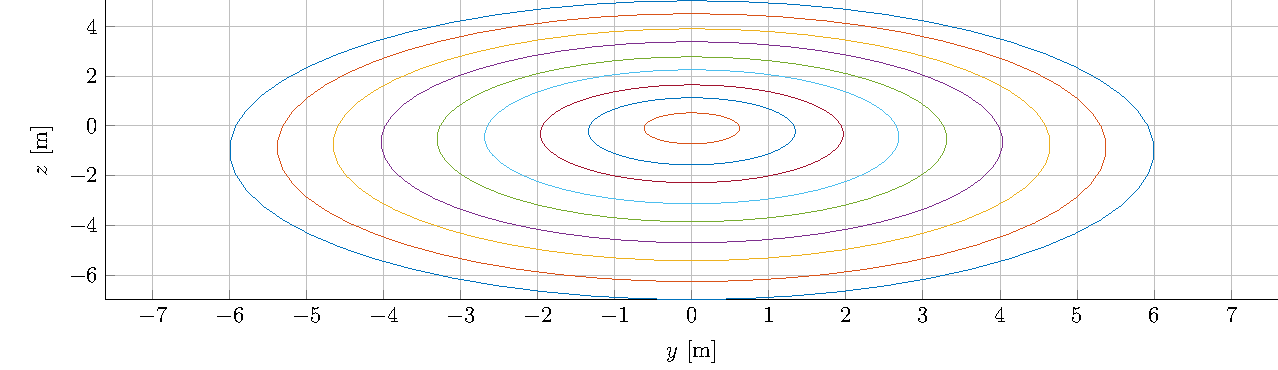
\includegraphics[width=0.99\textwidth]{./Figure/Aerodynamics/frontview.pdf}
		\caption{Front view}
		\label{fig:aeroshape.frontview}
	\end{subfigure}
	\begin{subfigure}[b]{0.49\textwidth}
		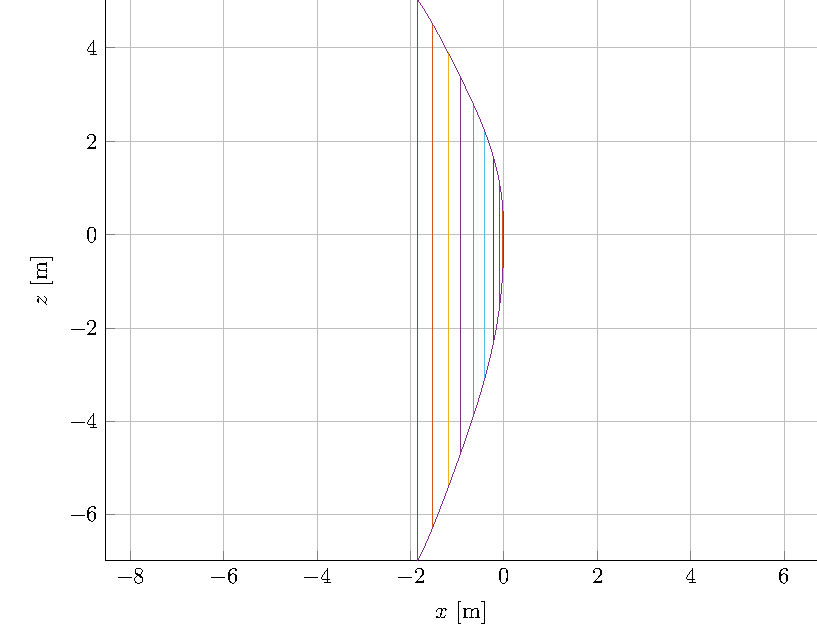
\includegraphics[width=0.99\textwidth]{./Figure/Aerodynamics/sideview.pdf}
		\caption{Side view}
		\label{fig:aeroshape.sideview}
	\end{subfigure}
	\begin{subfigure}[b]{0.49\textwidth}
		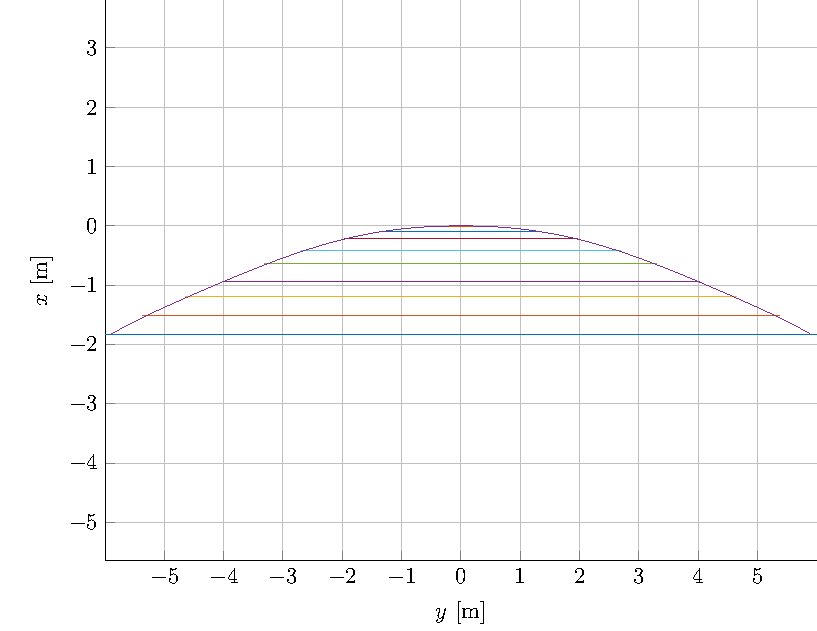
\includegraphics[width=0.99\textwidth]{./Figure/Aerodynamics/topview.pdf}
		\caption{Top view}
		\label{fig:aeroshape.topview}
	\end{subfigure}
	\begin{subfigure}[b]{0.49\textwidth}
		\includegraphics[width=0.99\textwidth]{./Figure/Aerodynamics/geometry_cp.eps}
		\caption{3D view}
		\label{fig:aeroshape.isoview}
	\end{subfigure}
	\caption{Front, side, top and 3D view of the inflatable shape}
\end{figure}
 
 Figures \ref{fig:CLCDCSAlpha} through \ref{fig:CGOAlpha} display the aerodynamic characteristics of the vehicle through an angle of attack range of $0 \left[deg\right]<\alpha<30 \left[deg\right]$. As can be seen from these plots, the behaviour of the lift-to-drag ratio and the moment coefficient in pitch is near linear. This linearity ensures predictable vehicle behaviour over the entire angle of attack range.
 
 \begin{figure}[h]
 	\centering
 	
 	\begin{subfigure}[b]{0.49\textwidth}
 		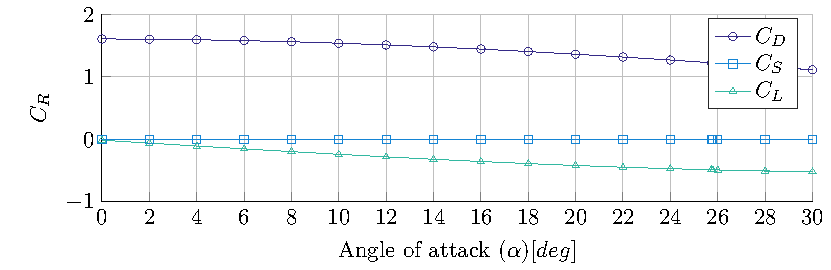
\includegraphics[width=0.99\textwidth]{./Figure/Aerodynamics/CDCSCLAlpha.pdf}
 		\caption{Force coefficients in the aerodynamic frame versus angle of attack}
 		\label{fig:CLCDCSAlpha}
 	\end{subfigure}
 	\begin{subfigure}[b]{0.49\textwidth}
 		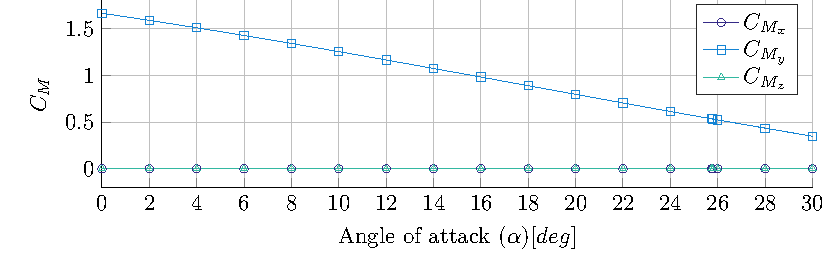
\includegraphics[width=0.99\textwidth]{./Figure/Aerodynamics/CMXCMYCMZAlpha.pdf}
 		\caption{Moment coefficients in the body frame versus angle of attack}
 		\label{fig:CMxCMyCMzAlpha}
 	\end{subfigure}
 	\begin{subfigure}[b]{0.49\textwidth}
 		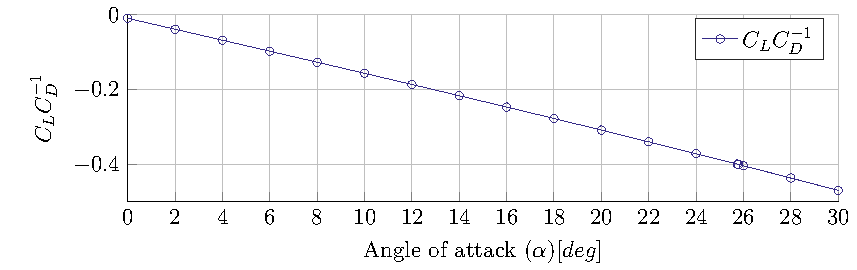
\includegraphics[width=0.99\textwidth]{./Figure/Aerodynamics/CLCDAlpha.pdf}
 		\caption{Lift-to-drag ratio versus angle of attack}
 		\label{fig:CLCDAlpha}
 	\end{subfigure}
 	\begin{subfigure}[b]{0.49\textwidth}
 		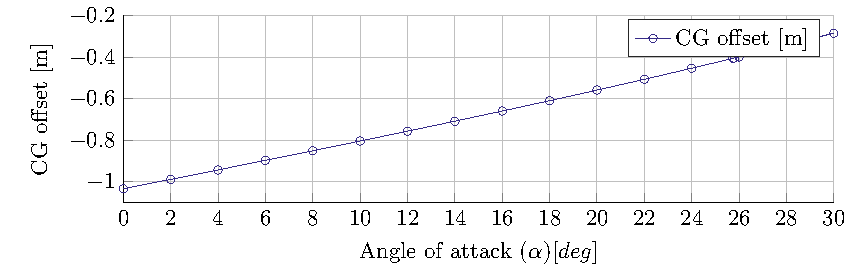
\includegraphics[width=0.99\textwidth]{./Figure/Aerodynamics/CGoAlpha.pdf}
 		\caption{Required \gls{cg}-offset versus angle of attack}
 		\label{fig:CGOAlpha}
 	\end{subfigure}
 	\caption{Various aerodynamic characteristics of the aeroshell over the angle of attack range $0 \left[deg\right]<\alpha<30 \left[deg\right]$}
 \end{figure}

\paragraph{Structural analysis and design}
The inflatable consists of ten toroids, stacked aside and on top of one another. The asymmetric shape obtained by aerodynamic optimisation is attained by arranging the toroids at an angle with respect to one another. The result is an assembly of circular inflatables, placed at differing radial distances with respect to the centre body. While the structural performance of the inflatable is altered, an asymmetric configuration is achieved by stitching the toroids and varying the radial length of the straps over the sphere cone circumference. Structural performance is altered in the sense that the asymmetry of the configuration implies additional concerns for aero-elastic phenomena, such as limit cycle oscillations, for example. These phenomena, however, are highly unpredictable and warrant additional wind tunnel and flight testing in any case. 

The number of toroids is based on Figure \ref{fig:inflpress_strucmass}, which shows that mass decreases beyond ten toroids are insignificant. Moreover, ten toroids are sufficient to adequately represent the optimised aerodynamic shape. 

Structural loads are carried by PBO Zylon\textsuperscript{\textregistered} fibres, interlaced warp and weft to provide load-carrying capability in all required directions: circumferential and hoop. As such,fibres are woven perpendicular to each other. To this end, a plain weave pattern is adequate.

For the load analysis, the ultimate load is calculated by multiplying the limit load, a peak dynamic pressure of $2300 \left[Pa\right]$ (with a $10\%$ density deviation from the nominal density), with a \acrfull{fos} of $1.5$. This \gls{fos} respects NASA standards for composite structures and accounts for uncertainties in the maximum external loading applied \cite{Technical2014}.  
From Figure \ref{fig:mat} and the parametric mass model it follows that for this ultimate load Vectran and aramid fibres Kevlar and Technora have exceeded their minimum gage thickness, set at $0.125 \left[mm\right]$ for aramid fibres. 

Such a minimum thickness is achievable for a plain weave, based on its proposed application in \gls{irve}-4 in a $0.127 \left[mm\right]$ lay-up \cite{Litton2011} and commercial availability of these weave patterns for Kevlar\footnote{URL: \url{http://www.cstsales.com/aramid_fabric.html}. Accessed: 16-06-2015}. Based on available grades of Vectran\footnote{URL: \url{http://www.swicofil.com/vectran.html\#Grades}. Accessed: 17-06-2015}, its minimum thickness is set at $0.023 \left[mm\right]$. PBO Zylon\textsuperscript{\textregistered}, on the other hand, remains at its minimum gage thickness for this loading. This minimum thickness is assumed to be the same as that of Kevlar, an assumption supported by the same yarn count and sample thickness in a study on ballistic impact on Kevlar 49 and PBO Zylon\textsuperscript{\textregistered} \cite{Pereira2009}. 

PBO Zylon\textsuperscript{\textregistered} offers a mass advantage of approximately $5 \left[kg\right]$ with respect to Technora and Vectran and $10 \left[kg\right]$ with respect to Kevlar. This mass advantage is the first reason for opting for PBO Zylon\textsuperscript{\textregistered}. In addition, PBO Zylon\textsuperscript{\textregistered} is capable of withstanding higher temperatures, $400 \left[^{\circ}C\right]$ for short exposure versus $250 \left[^{\circ}C\right]$ for Kevlar 49, one of the key drivers for its implementation in the upcoming \gls{thor} mission \cite{Dillman2014}. While in principle this would allow for a lighter \gls{tps}, this advantage is included as an additional contingency. At this stage, PBO Zylon\textsuperscript{\textregistered} fibres have not been applied in previous \gls{hiad} missions, in contrast to Kevlar 49 fibres. Since the mass limit is not exceeded, the mass advantage is not required and reliability is preferred due to the criticality of the inflatable. 

%Key driver for the design case at hand is the minimum material thickness: the loading was thusly low that the required thickness to withstand loads induced by aerodynamic and inflation pressure is lower than minimum gage thicknesses. To this end, fibre weight performance is mainly dictated by density and minimum gage thickness. The flexible material mass achieved by Spectra 2000, expected to perform best of all fibres given its low density of 970 [$kg \cdot m^{-3}$], compared to Kevlar's 1440 [$kg \cdot m^{-3}$], is 20 [$kg$] lower than that achieved by Kevlar 49 and the other fibres, of comparable density. 

%Preference is given to Kevlar 49, however, for two reasons. Firstly, it is widely commercially available and has been applied for a longer number of years, with resulting lower costs associated with its fabrication and application. Secondly, it has been previously applied for inflatable re-entry vehicles, namely in the \gls{irve} missions \cite{Hughes2011}. Spectra 2000 therefore introduces additional costs and technical risks that offset the weight advantage offered. Moreover, the weight advantage does not further the entry vehicle in the sense that supplementing another crew member is out of reach and requirements are respected. Other fibres are comparable to Kevlar in their performance, with none of the benefits of past application in \glspl{hiad}.

%Based on the parametric mass model and the inherent stress equations, the minimum gage thickness of 0.125 [$mm$] is deemed attainable. Such a minimum thickness is achievable for a plain weave, based on its proposed application in \gls{irve}-4 in a 0.127 [$mm$] lay-up \cite{Litton2011} and commercial availability of these weave patterns\footnote{URL:\url{http://www.cstsales.com/aramid_fabric.html}. Accessed: 16-06-2015}. 

The structural feasibility of the configuration is ascertained by the truss-based analysis model. The truss-based analysis model uses the representation in Figure \ref{fig:strucreps}. Cross-sections that displayed the most extreme loading are the short side, defined at the inflatable minimum diameter, and the long side, defined at the inflatable maximum diameter. Due to the skewness, load asymmetry is introduced which is thereby evaluated by some extent through evaluation of multiple cross-sections.

\begin{figure}[h]
	\centering

	\begin{subfigure}[b]{0.45\textwidth}
		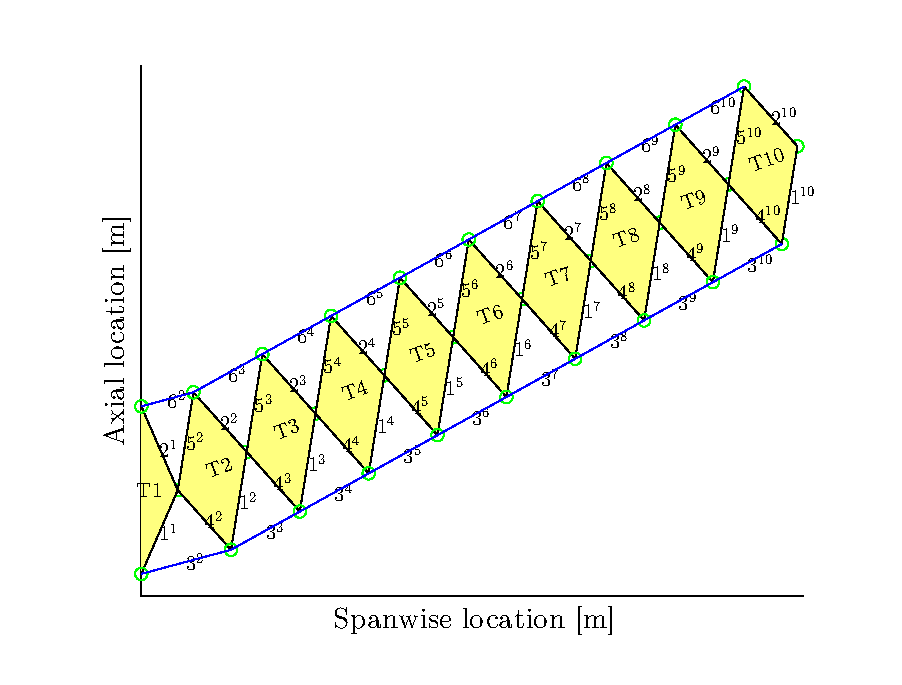
\includegraphics[width=0.96\textwidth]{./Figure/Structure/shape_long.eps}
		\caption{Cross-sectional view at maximum diameter}
		\label{fig:shapel}
	\end{subfigure}
	\begin{subfigure}[b]{0.45\textwidth}
		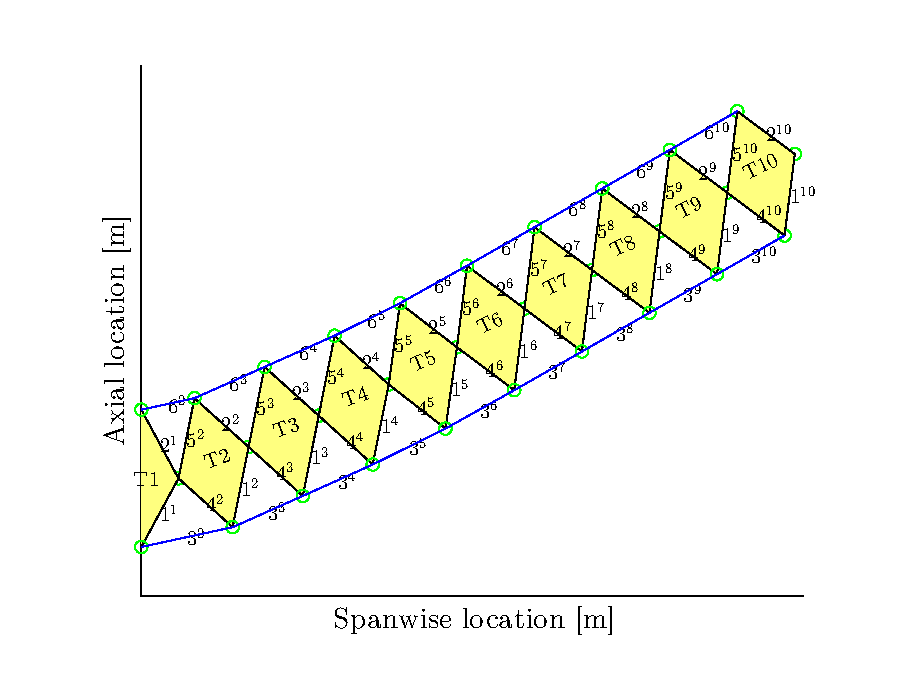
\includegraphics[width=0.96\textwidth]{./Figure/Structure/shape_short.eps}
		\caption{Cross-sectional view at minimum diameter}
		\label{fig:shapes}
	\end{subfigure}
\begin{subfigure}[c]{0.5\textwidth}
		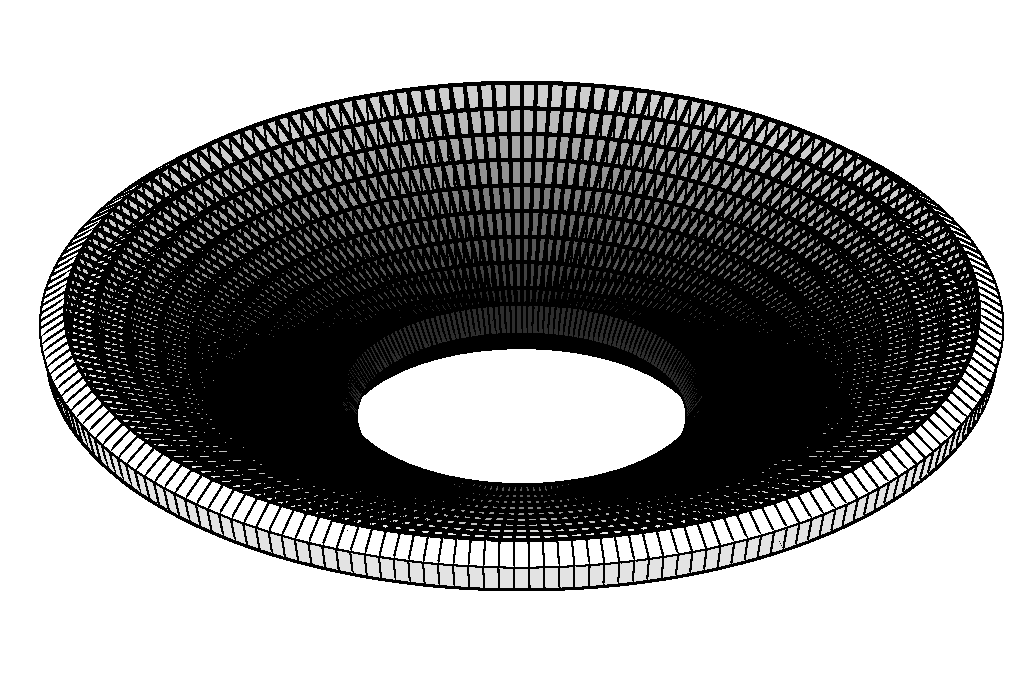
\includegraphics[width=0.96\textwidth]{./Figure/Structure/struc_rep.eps}
		\caption{Isometric view}
		\label{fig:iso}
	\end{subfigure}
\caption{Structural representation of inflatable structure}
\label{fig:strucreps}
\end{figure}

For an inflation pressure of $169 \left[kPa\right]$, required to bring all members into tension, structural loads are as obtained in Figures \ref{fig:strucl} and \ref{fig:strucs}. It can be observed that the maximum running load in the walls is $50 \left[kN \cdot m^{-1}\right]$. Translating this to a stress by dividing through the $0.125 \left[mm\right]$ thickness yields a maximum stress of $400 \right[MPa\right]$, well below the (room-temperature) tensile strength of $5.8 \left[GPa\right]$ for PBO Zylon\textsuperscript{\textregistered}. In the straps, the maximum running load is $100 \left[kN \cdot m^{-1}\right]$, translating to a $800 \left[MPa\right]$ stress. As such, the minimum gage thickness is well above the required thickness determined by preliminary load and stress analysis. Firstly this takes into account material strength loss at higher temperatures, as PBO Zylon\textsuperscript{\textregistered} retains $80\%$ of its strength when exposed to $200 \left[^{\circ}C\right]$. Secondly, it takes into account a wide margin for material uncertainties, production deficiencies and unpredicted structural phenomena. The flexible material mass, given a uniform thickness of $0.125 \left[mm\right]$ for radial straps and toroid material, is $110 \left[kg\right]$.

\begin{figure}[h]
		\hspace{-16mm}
		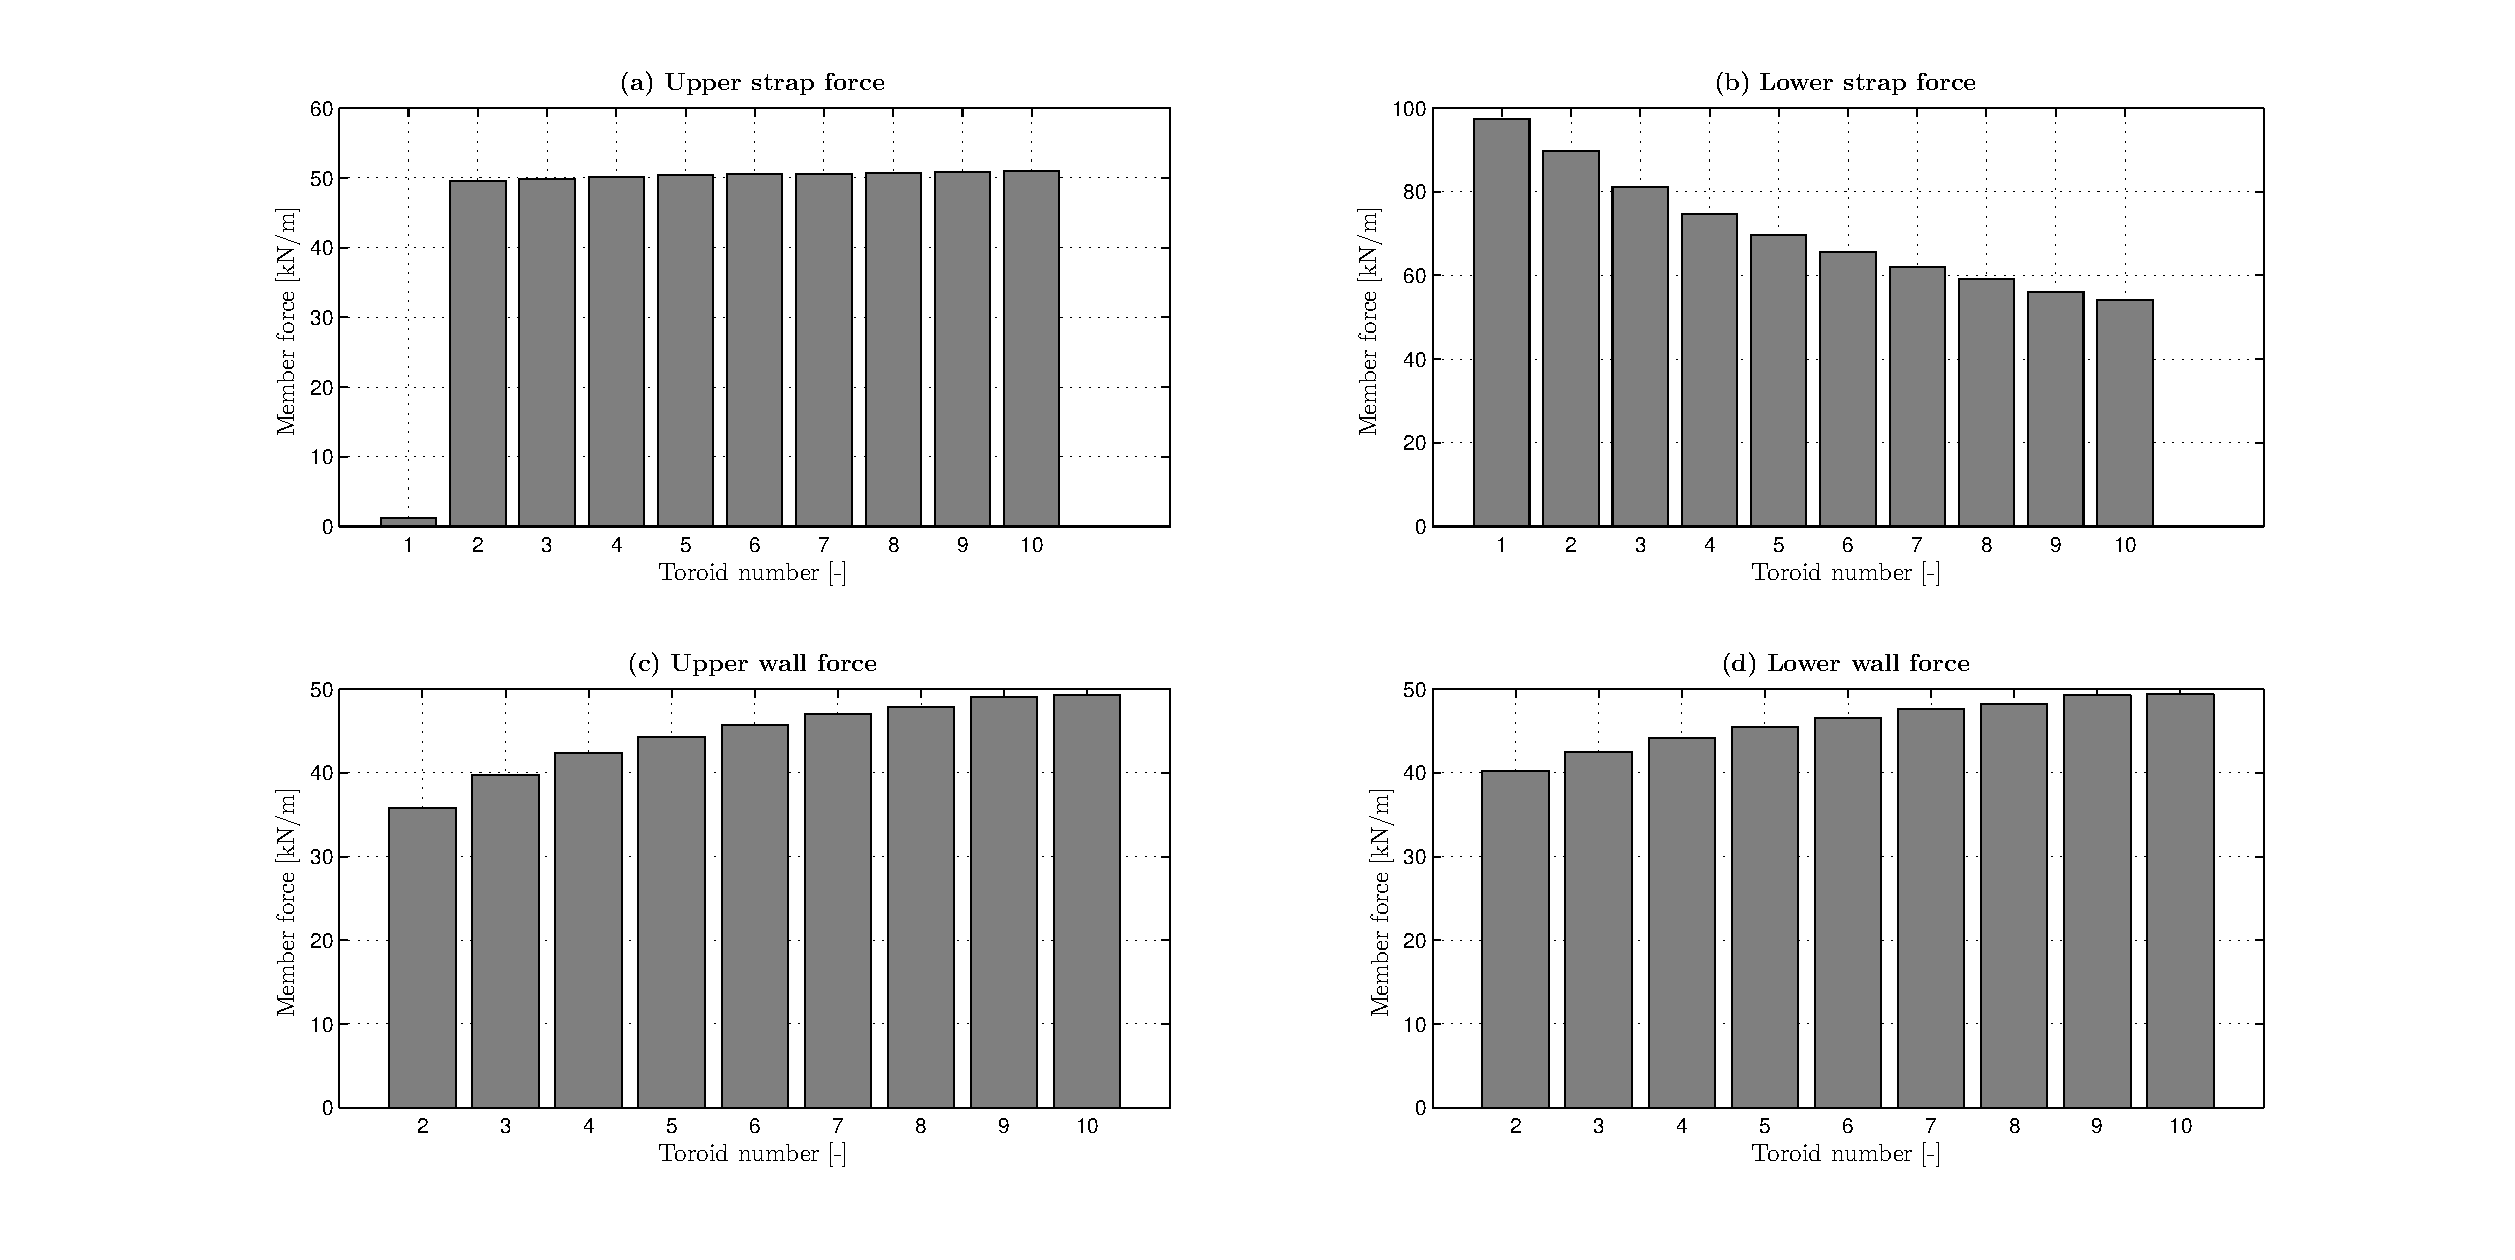
\includegraphics[width=1.2\textwidth]{./Figure/Structure/loads_long.eps}
		\caption{Cross-sectional running loads inflatable at maximum diameter}
		\label{fig:strucl}
\end{figure}
\begin{figure}[h]
		\hspace{-16mm}
		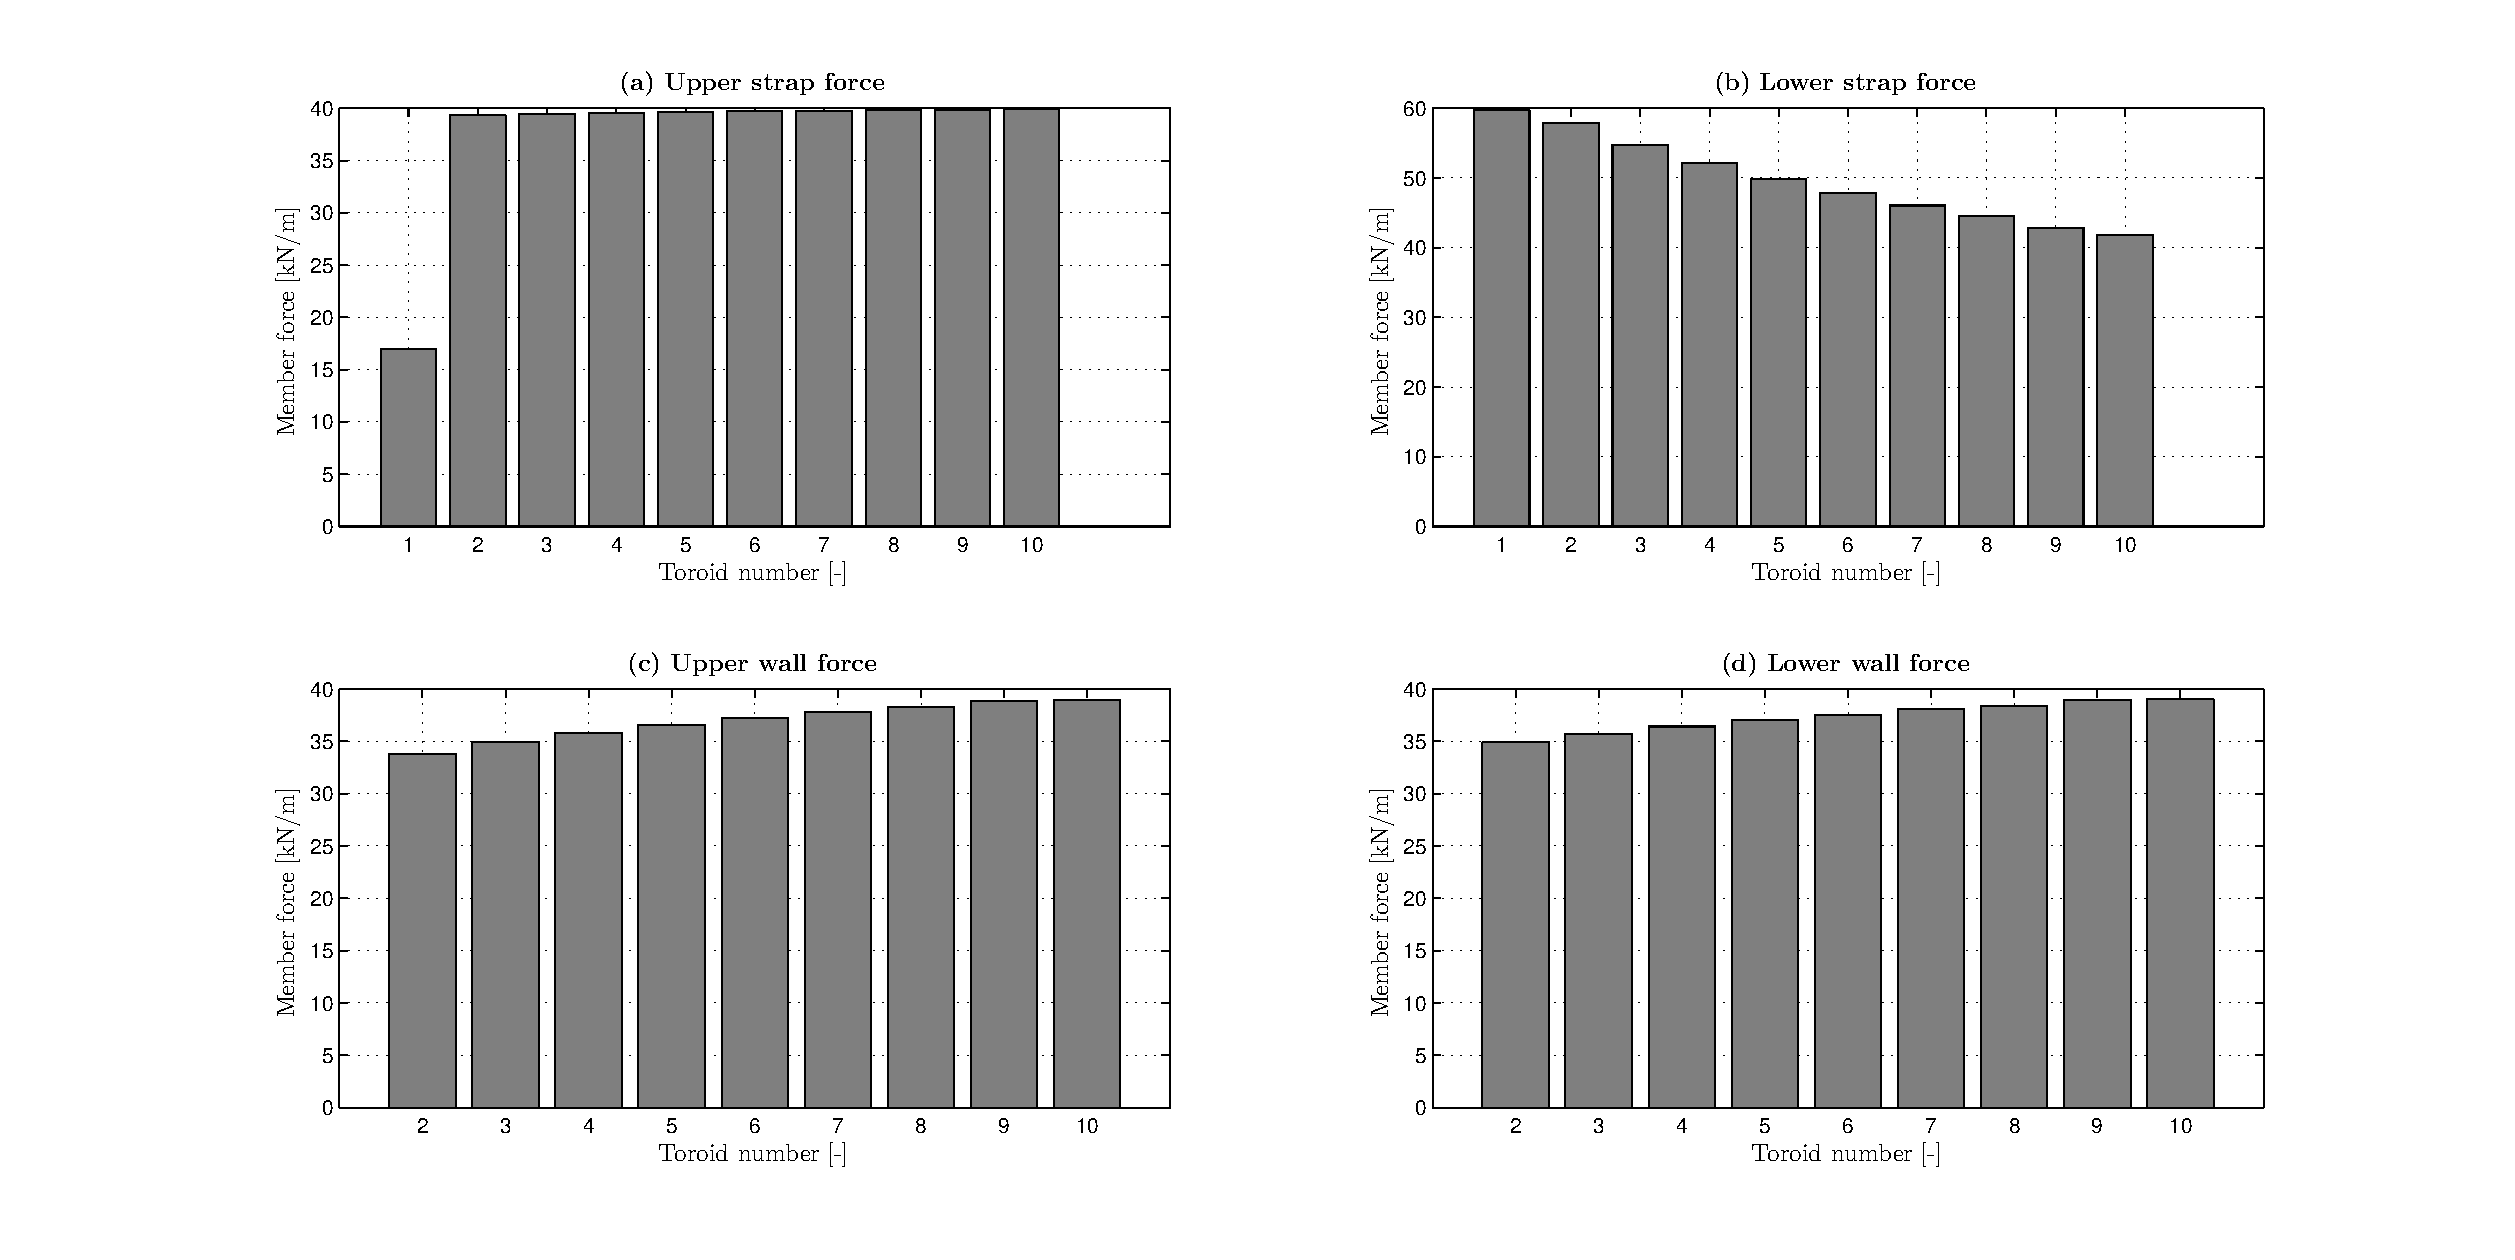
\includegraphics[width=1.2\textwidth]{./Figure/Structure/loads_short.eps}
		\caption{Cross-sectional running loads inflatable at minimum diameter}
		\label{fig:strucs}
\end{figure}

Stitching of the fabrics making up the toroids is used for the joints of the inflatable, on one hand to join the toroids to each other and on the other hand to join the toroids to the radial straps. This is a method excellently suited, applied, tested and proven in the \gls{irve} missions \cite{Lindell2006,Hughes2011,Dillman2012}. Joints are thereby proven high-strength and suitable for space application and a stacked-toroid configuration.

To prevent the inflation gas from leaking, the structural PBO Zylon\textsuperscript{\textregistered} layers are coated with a gas barrier in the form of a $50 \left[\mu m\right]$ Upilex layer. This uniform thickness coating adds an estimated $25 \left[kg\right]$. The thickness of this coating is feasible, in line with findings by Samareh and Miller \cite{Samareh2011,Miller2014} and available Upilex grades of $12.5$, $25$, $50$, $75$ and $125 \left[\mu m\right]$\footnote{URL: \url{https://www.ube.com/content.php?pageid=81}. Accessed: 16-06-2015}$^{,}$\footnote{URL: \url{http://dasp.mem.odu.edu:8080/~deorbit_sp12/ref/UPILEXS\%20Data\%20sheet.pdf}. Accessed: 16-06-2015}.

%Typical driver for the use of fibres are the high mechanical properties, hence the application of Kevlar in the \gls{irve} missions \cite{Hughes2011}. Structural analyses proved the weight advantage of fibres over films in the case of \gls{irve}. In this case, however, density is leading and the mechanical properties of fibres are excessively high: their application would lead to an overdesign. This is reflected by Table \ref{tab:matfinal}. The flexible material mass achieved by Spectra 2000, expected to perform best of all fibres given its low density of 970 [$kg \cdot m^{-3}$], compared to Kevlar's 1440 [$kg \cdot m^{-3}$], is 20 [$kg$] lower than that achieved by Kevlar 49. 

%Films, however, provide a significant weight advantage. Upilex-25S and Kapton are films suitable for \gls{hiad} application \cite[p.59]{Balasooriyan2015b}. Upilex-25S is characterized by higher mechanical properties than Kapton, and due to the low minimum thickness for these films specific strength is the leading material property. The specific strength of Upilex-25S is nearly twice as high as that of Kapton \cite{Samareh2011} and this is reflected by its mass, nearly twice as low. The predominant advantage of using Upilex-25S over fibres is therefore directly reflected by the lower achievable structural mass, yielding a flexible material mass of 30 [$kg$].
%\begin{table}[h]
%\centering
%\caption{Comparison of flexible material mass for use of different materials}
%\label{tab:matfinal}
%\begin{tabular}{|l|l|l|l|l|}
%\hline
%{\bf Material}                        & Kevlar 49    & Spectra 2000 & Upilex-25S & Kapton \\ \hline
%{\bf Type}                            & Aramid fibre & Aramid fibre & Film       & Film   \\ \hline
%{\bf Flexible material mass {[}kg{]}} & 89             &  71          &  31          & 52        \\ \hline
%\end{tabular}
%\end{table}

%The weight advantage is predominantly effected by a lower minimum gage thickness for films. Minimum gage thickness for Upilex-25S is 25 [$\mu m$]\footnote{URL:\url{http://dasp.mem.odu.edu:8080/~deorbit_sp12/ref/UPILEXS\%20Data\%20sheet.pdf}. Accessed: 16-06-2015}.  The thickness required to withstand the loads is estimated at 0.025 [$mm$]



%As such, based on the discussion in Subsection \ref{subsec:strucsens} Spectra 2000 is expected to perform best given its low density of 970 [$kg \cdot m^{-3}$], compared to Kevlar's 1440 [$kg \cdot m^{-3}$]. This effects a 20 [$kg$] decrease in material mass by the use of Spectra 2000 as compared to the other materials in Figure \ref{fig:mat}, of comparable density with Kevlar 49. 

%Stitching of the fabrics making up the toroids is used for the joints of the inflatable, on one hand to join the toroids to each other and on the other hand to join the toroids to the radial straps. This is a method excellently suited, applied, tested and proven in the \gls{irve} missions \cite{Lindell2006,Hughes2011,Dillman2012}. Joints are thereby proven high-strength and suitable for space application and a stacked-toroid configuration.

%Structural integrity is provided by PBO Zylon AS, capable of retaining its strength at high temperature and able to withstand the required loads\footnote{URL:\url{http://www.toyobo-global.com/seihin/kc/pbo/zylon-p/bussei-p/technical.pdf}. Accessed: 15-06-2015}}. It has high specific properties, leading to a low structural mass, as follows from Figure \ref{fig:mat}. It performs only slightly worse than Spectra 2000 in the parametric mass model, but differences are slight (below 5 $\%$) and 

\clearpage

\paragraph{\acrlong{tps} design}
For a given trajectory and lay-up it is possible to check the temperature distribution for failure. From the sensitivity analysis in Section \ref{subsec:thermalsens} it is deducted that a Nextel BF-20 layer with Pyrogel\textsuperscript{\textregistered} 6650 as insulator is preferable for mass reduction purposes. However, due to the relatively low emissivity of Nextel the wall temperature exceeds the limit as high aerodynamic heating can not be radiated away efficiently. For this reason a slightly heavier alternative, Nicalon\textsuperscript{TM}, is needed. Nicalon\textsuperscript{TM} is a type of silicon continuous fibre that can withstand temperatures up to $2073 \left[K\right]$. Furthermore it has a much higher emissivity, which greatly reduces the wall temperature. It performs comparable or even better on its ability fold compared with Nextel BF-20 \cite{Corso2011}. The sensitivity analysis has shown that for a diameter of $12 \left[m\right]$ it was not possible to find a viable thickness for the Nextel lay-ups. Several iterations have been performed to reduce the heat flux such that Nextel BF-20 became viable, however these attempts resulted only in an approximate mass of $500 \left[kg\right]$. Therefore Nicalon\textsuperscript{TM} is chosen as \gls{tps}-layer and Pyrogel\textsuperscript{\textregistered} 6650 as insulation layer for the lay-up in the final design. In addition to the Upilex coating on the inside of the PBO Zylon\textsuperscript{\textregistered} layer, two thin impermeable layers of kapton are placed between the Pyrogel\textsuperscript{\textregistered} and Zylon\textsuperscript{\textregistered} to prevent hot gasses reaching the Zylon\textsuperscript{\textregistered} layer \cite{Hughes2005,Litton2011}.

The incoming heat flux, or aerodynamic heating of the chosen trajectory is shown in Figure \ref{fig:heatfluxes}. The heat maximum heat flux is approximately $21 \left[W\cdot cm^{-2}\right]$. The maximum heat flux for the entry phase is $7.3 \left[W\cdot cm^{-2}\right]$. It is expected that this entry phase is not leading for the design and therefore it is not shown. In the figure three fluxes are shown for the aerocapture phase, which represent the change in heat flux when the atmospheric density is over- or underestimated by $10\%$. This $10\%$ comes from the uncertainties in the density as explained in Section \ref{sec:trajectorydesign}. Surprisingly, when the density is underestimated by $10\%$, the heat load becomes slightly higher as the duration of the trajectory is longer and this results in a higher required thickness. This case is used as reference heat flux for which the lay-up is optimised.

\begin{figure}[h]
	\centering
	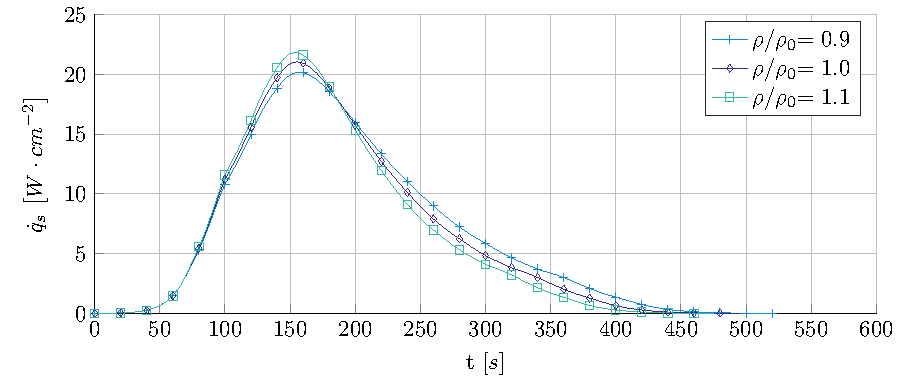
\includegraphics{./Figure/Thermal/heatfluxes.pdf}
	\caption{Heat flux of the aerocapture for different density levels}
	\label{fig:heatfluxes}
\end{figure}

Figures \ref{fig:thermoaero} and \ref{fig:thermoentry} show how the heat propagates though the material during the aerocapture and entry phase of the chosen trajectory. It is clear that the aerocapture is indeed leading for the design as the heat load during this phase and resulting temperatures are higher. The figure can also be used to understand the required thicknesses. The Nicalon\textsuperscript{TM} and Pyrogel\textsuperscript{\textregistered} layers remain far below their maximum temperatures, $2073 \left[K\right]$ and $923 \left[K\right]$ respectively. Therefore the Nicalon\textsuperscript{TM} layer is as thin as possible, which is $0.508 \left[mm\right]$. For the kapton and PBO Zylon\textsuperscript{\textregistered} layers the maximum temperature is set at $473 \left[K\right]$ to remain their structural integrity. This is why the insulation layer is needed such that the temperature drops to this maximum through the Pyrogel\textsuperscript{\textregistered} 6650. The required thickness for this is $2.439 \left[mm\right]$. Each kapton layer is also very thin which comes down to $0.025 \left[mm\right]$.

\begin{figure}[h]
	\centering
	\begin{subfigure}[b]{0.45\textwidth}
		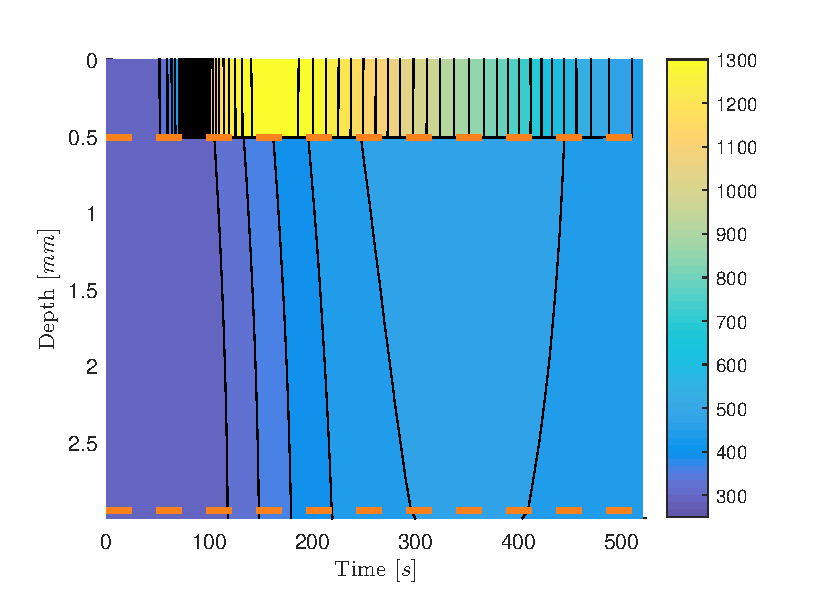
\includegraphics[width=\textwidth]{./Figure/Thermal/Thermal_contour_capture.eps}
		\caption{Aerocapture}
		\label{fig:thermoaero}
	\end{subfigure}
	~ %add desired spacing between images, e. g. ~, \quad, \qquad, \hfill etc.
	%(or a blank line to force the subfigure onto a new line)
	\begin{subfigure}[b]{0.45\textwidth}
		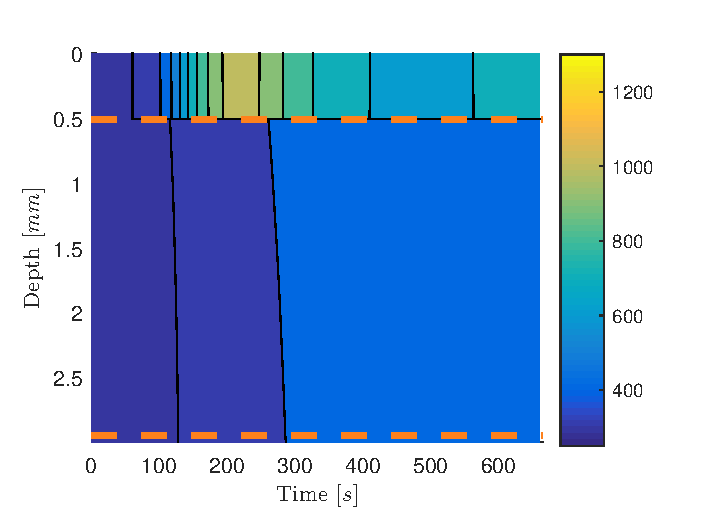
\includegraphics[width=\textwidth]{./Figure/Thermal/Thermal_contour_entry.eps}
		\caption{Entry}
		\label{fig:thermoentry}
	\end{subfigure}
	\caption{Heat propagation during both decelerations}\label{fig:heatprop}
\end{figure}

The areal density of this lay-up is $1.816 \left[kg\cdot m^{-2}\right]$. The frontal surface area or wetted area is $120.9 \left[m^2\right]$, as is obtained from the aerodynamic analysis. Multiplying the surface area with the area density results in a frontal \gls{tps} mass of $219.6 \left[kg\right]$. Note that the frontal \gls{tps} covers the rigid centre body of the vehicle. For the protection on the other side of the inflatable very thin layers of kapton and Nextel AF-14 are assumed to be sufficient. The resulting area density is $0.342 \left[kg\cdot m^{-2}\right]$. The area onto which it is applied is assumed to be the frontal surface area minus the centre body area, which equals to $105.0 \left[m^2\right]$. The resulting mass is $35.96 \left[kg\right]$. The total \gls{tps} mass for the lay-up shown in Figure \ref{fig:finallayup} yields $255.6 \left[kg\right]$. 

\begin{figure}[H]
	\centering
	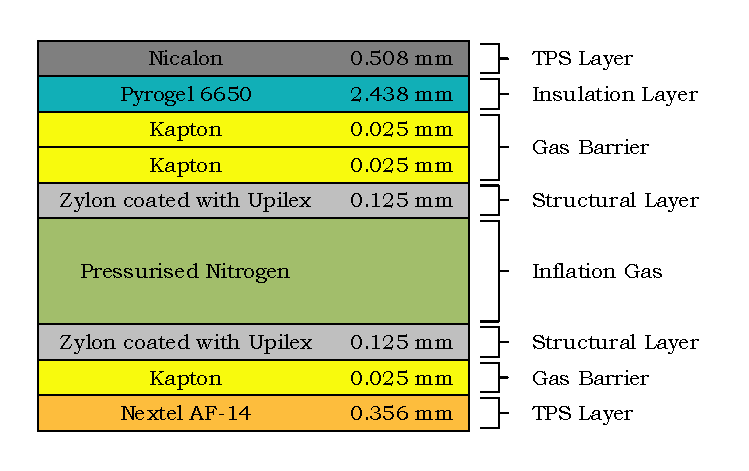
\includegraphics{./Figure/Thermal/finallayup.pdf}
	\caption{Final design for the \acrlong{tps}}
	\label{fig:finallayup}
\end{figure}
